\documentclass[a4paper]{article}

% Simple margin hack from
%   http://kb.mit.edu/confluence/pages/viewpage.action?pageId=3907057
\usepackage[margin=2cm]{geometry}

\usepackage{graphicx}       % Extended support for \includegraphics
\usepackage{tikz}           % Powerful drawing package, part of pgf

\usepackage{mathptmx}       % Mathematical PostScript fonts
\usepackage{amsmath}        % General mathematical symbols
\usepackage{textcomp}       % Text companion fonts

\usepackage{url}            % \url command for decent line breaks in urls
\usepackage{enumitem}       % For more control over list parameters.

\usepackage{tabularx}       % tabularx environment
\usepackage{booktabs}       % Improved tables
\usepackage{multicol}       % Multiple columns inline


% Some paragraph tweaks from
%   https://www.sharelatex.com/learn/Paragraph_formatting
\setlength\parindent{0pt}
\setlength\parskip{0.5em}

\setlength\extrarowheight{2pt}

% Tone down hyphenation and allow lines to stretch in compensation
\hyphenpenalty 4000
\sloppy


% PGF and TikZ definitions for this paper

% TikZ library imports
\usetikzlibrary{positioning}        % Anchor placement support
\usetikzlibrary{calc}               % Coordinate calculations
\usetikzlibrary{shapes.geometric}   % cylinder
\usetikzlibrary{shapes.arrows}      % arrow shapes
\usetikzlibrary{shapes.multipart}
\usetikzlibrary{fit}                % Fitting outline to shape
\usetikzlibrary{arrows}
\usetikzlibrary{arrows.meta}
\usetikzlibrary{shadows}


% Define our colours
\colorlet{normal colour}{green!60!blue!20}  % Normal coloured filled areas
\colorlet{accent colour}{orange!25}         % Accented filled areas
\colorlet{background colour}{black!10}      % Background groups
\colorlet{data colour}{black!50}            % Data flow
\colorlet{trigger colour}{black!80}         % Trigger lines
\colorlet{control colour}{blue!50}          % Other lines etc


% Common TikZ definitions
\tikzset{
    % This seems a reasonably comfortable arrow shape
    >=stealth,
%
    % Define a set of styles
    % First some fills
    background fill/.style={fill=background colour},
    highlight fill/.style={fill=normal colour},
    accent fill/.style={fill=accent colour},
    % Next some lines
    bus/.style={color=data colour, text=black, line width=0.6mm, ->},
    control/.style={color=control colour, text=black, very thick, ->},
%
    % Used for creating an exact fit to an existing list of objects
    tight fit/.style={fit=#1, inner sep=0, line width=0},
    % We almost always want centre aligned node text
    every node/.style={align=center},
%
    box/.style={
        draw, rectangle, very thick, highlight fill,
        minimum width=1.5cm, minimum height=1.1cm},
    small box/.style={
        draw, rectangle, thick, highlight fill},
    component/.style={
        draw, rectangle, thick, accent fill,
        minimum width=11mm, minimum height=8mm},
    buffer/.style={
        regular polygon, regular polygon sides=3, anchor=center,
        accent fill, thick, draw},
    generate/.style={
        background fill, thin, draw=gray,
        copy shadow={
            shadow xshift=1ex, shadow yshift=-1ex}},
%
    trigger line/.style={thin, trigger colour},
    trigger/.style={
        trigger line, >={Triangle[open, scale=1.2]}, shorten >=-5pt, ->},
    trigger dot/.style={fill, circle, inner sep=1pt, line width=-1pt},
%
    inline text/.style={
        baseline=(current bounding box.base),
        every node/.append style={anchor=base, font=\scriptsize},},
%
    pics/buffer/.style args={#1/#2}{
        code={
            \draw [thick, -, black] (0.5mm,-2mm) -- (0.5mm,2mm);
            \draw [thick, -, black] (-0.5mm,-2mm) -- (-0.5mm,2mm);
            \node at (0,2mm) [
                rotated anchor=-90, font=\scriptsize, inner sep=0.2em] {#1}
            node at (0,-2mm) [
                rotated anchor=90, font=\scriptsize, inner sep=0.2em] {#2};}},
}


% New tikz key definitions to control behaviour of \multipath.
\tikzset{
    % Default colour for multipath background
    multipath background/.initial=white,
    multipath margin/.initial=0.3mm,
}

% Draws multiple paths with an outline on each path.  Call with path options as
% first optional argument and with a list of paths as the second argument.
\newcommand{\multipath}[2][]{
    \begin{scope}[#1]
        % Pick up multipath margin and background definitions
        \newcommand{\margin}{\pgfkeysvalueof{/tikz/multipath margin}}
        \newcommand{\background}{\pgfkeysvalueof{/tikz/multipath background}}

        % Draw a white background a bit larger than the programmed line
        % thickness.  We turn off any arrows and shorten the line a trifle to
        % avoid any erosion of the endpoints.
        \begin{scope}[
            line width=\pgflinewidth+\margin, color=\background,
            shorten >=\margin, shorten <=\margin, -]
        #2
        \end{scope}

        % Now draw the target path with its original options.
        #2
    \end{scope}
}

% Special coordinates along edge of box
\newcommand{\northcoord}[3]{
    \coordinate (#1 #2) at ($(#1.north west)!#3!(#1.north east)$)}
\newcommand{\eastcoord}[3]{
    \coordinate (#1 #2) at ($(#1.south east)!#3!(#1.north east)$)}
\newcommand{\southcoord}[3]{
    \coordinate (#1 #2) at ($(#1.south west)!#3!(#1.south east)$)}
\newcommand{\westcoord}[3]{
    \coordinate (#1 #2) at ($(#1.south west)!#3!(#1.north west)$)}


% Trick for reusing last coordinate
\makeatletter
\newcommand\lastcoord{\the\tikz@lastxsaved,\the\tikz@lastysaved}
\makeatother


% It's convenient to have a background layer
\pgfdeclarelayer{background}
\pgfsetlayers{background,main}



% ------------------------------------------------------------------------------
% This frightening looking code is used to compute an anchor that rotates with
% the entire picture.  This is useful when anchoring a node in a pic that itself
% will be rotated.
%   Some really tricky code taken from stack overflow question here:
%
%   https://tex.stackexchange.com/questions/128565/
%       how-to-allow-labels-anchors-in-tikz-to-be-affected-by-
%       rotations-without-rotatin

% \pgfmath@smuggleone
%
% Smuggle a macro outside a group.
%
% Changed by TT: Speedup by insisting, that smuggleone is directly
% followed by \endgroup
%
\makeatletter
\def\pgfmath@smuggleone#1\endgroup{%
  \expandafter\endgroup\expandafter\def\expandafter#1\expandafter{#1}}

\let\pgfmathsmuggle=\pgfmath@smuggleone
\makeatother

\tikzset{
    rotated anchor/.code=%
        \begingroup
            \pgfcoordinate{qrr@origin}{\pgfpointorigin}%
            \pgfcoordinate{qrr@direct}{\pgfpointpolarxy{#1}{1}}%
            \pgftransformreset
            \pgfmathanglebetweenpoints{%
                \pgfpointanchor{qrr@origin}{center}}{%
                    \pgfpointanchor{qrr@direct}{center}}%
            \pgfmathsmuggle\pgfmathresult
        \endgroup
    \tikzset{anchor/.expanded=\pgfmathresult}%
}

% ------------------------------------------------------------------------------

% vim: set filetype=tex:



\begin{document}



\begin{figure}[ht]
\begin{centering}
\newcommand{\drawpin}[2]{
    \draw [thick] (#2) -- (#2|-#1.south) coordinate (circle);
    \draw [thick, fill=white] (circle) circle (3pt);}

\begin{tikzpicture}

    % Nodes:
    %   interconnect
    %   axi burst master
    %   axi lite slave
    \path
        node [box, minimum width=5cm] (interconnect) {interconnect}
        ++(0,-2.5) node [box] (axi burst master) {axi burst\\master}
        +(-3.5,0) node [box] (axi lite slave) {axi lite\\slave};

    % Interconnect end points
    \northcoord{interconnect}{PCIe out}{0.15};
    \northcoord{interconnect}{DRAM0 out}{0.5};
    \northcoord{interconnect}{DRAM1 out}{0.85};
    \southcoord{interconnect}{lite slave}{0.15};
    \southcoord{interconnect}{burst master}{0.5};
    \southcoord{interconnect}{lite master}{0.85};

    % Nodes:
    %   axi lite master
    %   register top
    %   system registers
    %   clocking
    %   dsp main
    \path (interconnect-|interconnect lite master)
        +(0,-2.5) node [box] (axi lite master) {axi lite\\master};
    \path (axi lite slave)
        ++(0,-1.5) node [box] (register top) {register\\top}
        ++(-3.5,0) node [box] (system registers) {system\\registers}
        ++(0,-2.5) node [box, minimum height=2cm] (clocking) {clocking};
    \path (axi burst master)
        ++(1,-3) node [box, minimum width=5cm, minimum height=3.5cm]
            (dsp main) {dsp main};

    % --------------------------------------------------------------------------
    % FMC 500M
    \path (interconnect)
        ++(-4.5,-10) node [
            background fill, minimum width=6cm, minimum height=3cm,
        ] (fmc500m) {};
    \node [below right, background fill] at (fmc500m.north west) {fmc500m};

    \path (fmc500m)
        ++(0,-0.4) node [component] (PLL) {PLL}
        +(-1.8,0) node [component] (ADC) {ADC}
        +(1.8,0) node [component] (DAC) {DAC};

    % Paths to ADC
    \drawpin{fmc500m}{ADC.-125}
    \node [anchor=north west, yshift=-3pt, xshift=-2mm, font=\small]
        at (circle) {ADC\textsubscript{in}};
    \drawpin{fmc500m}{ADC.-55}
    \draw [bus] (ADC) -- ++(0,1) -| (fmc500m.60);
    % Paths to DAC
    \drawpin{fmc500m}{DAC.-125}
    \node [anchor=north west, yshift=-3pt, xshift=-4mm, font=\small]
        at (circle) {DAC\textsubscript{out}};
    \drawpin{fmc500m}{DAC.-55}
    \draw [bus, <-] (DAC) -- ++(0,1) -| (DAC|-fmc500m.north);
    % Paths to PLL
    \drawpin{fmc500m}{PLL}
    \draw [trigger] ([yshift=2mm]circle) -- (PLL);
    \node [anchor=north, yshift=-3pt, font=\small]
        at (circle) {f\textsubscript{RF}};
    \draw [trigger] (PLL) -- (ADC);
    \draw [trigger] (PLL) -- (DAC);
    % Fast trigger
    \draw [thick, ->]
        ([xshift=-4mm]fmc500m.south east) coordinate (circle) --
        +(0,3.5) -| (dsp main.-120);
    \draw [thick, fill=white] (circle) circle (3pt);
    \node [anchor=north, yshift=-3pt, xshift=1mm, font=\small]
        at (circle) {f\textsubscript{REV}};
    % Place idelay
    \node [small box, yshift=35mm, xshift=10mm]
        at (circle) {idelay};

    \draw [trigger]
        (ADC) -- +(-2,0) |- ($(clocking.west)+(0,-0.55)$);
    \draw [trigger]
        ($(clocking.west)+(0,0.55)$)
        +(-1,0) node [anchor=south, font=\scriptsize, black] {125\,MHz}
        -- ($(clocking.west)+(0,0.55)$);


    % --------------------------------------------------------------------------
    % FMC digital IO
    \path (interconnect)
        ++(4,-10) node [
            background fill, minimum width=5cm, minimum height=3cm,
        ] (fmc digital io) {};
    % Buffers
    \draw (fmc digital io)
        ++(-1.8,-0.5) node [buffer] (buf1) {}
        ++(0.9,0) node [buffer] (buf2) {}
        ++(0.9,0) node [buffer] (buf3) {}
        ++(0.9,1.5mm) node [buffer, rotate=180] (buf4) {}
        ++(0.9,0) node [buffer, rotate=180] (buf5) {};
    \drawpin{fmc digital io}{buf1}
    \node [anchor=north, yshift=-3pt, font=\small] at (circle) {TRG};
    \drawpin{fmc digital io}{buf2}
    \node [anchor=north, yshift=-3pt, font=\small] at (circle) {PM};
    \drawpin{fmc digital io}{buf3}
    \node [anchor=north, yshift=-3pt, font=\small] at (circle) {BLK};
    \drawpin{fmc digital io}{buf4}
    \node [anchor=north, yshift=-3pt, font=\small] at (circle) {SEQ0};
    \drawpin{fmc digital io}{buf5}
    \node [anchor=north, yshift=-3pt, font=\small] at (circle) {SEQ1};
    \node [below right] at (fmc digital io.north west) {fmc digital io};

    \draw [thick, ->] (buf1) -- +(0,1) -| (fmc digital io.80);
    \draw [thick] (buf2) -- +(0,1);
    \draw [thick] (buf3) -- +(0,1);
    \draw [thick, <-] (buf4) -- +(0,1) -| (fmc digital io.50);
    \draw [thick, <-] (buf5) -- +(0,1) -| (fmc digital io.50);


    % --------------------------------------------------------------------------
    % Clocking links

    % REF clock
    \draw [trigger] ($(clocking.east)+(0,0.8)$)
        node [above right, font=\scriptsize, black] {REF\_CLK}
        -- ++(1,0)
        coordinate (REF CLK);

    % REG clock
    \draw [trigger line] ($(clocking.east)+(0,0.3)$)
        node [above right, font=\scriptsize, black] {REG\_CLK}
        -- ++(1.4,0) -- ++(0,1.9)
        node [trigger dot] {}
        coordinate (REG CLK);
    \draw [trigger] (REG CLK) -- (REG CLK-|system registers.east);
    \draw [trigger] (REG CLK) -- (REG CLK-|register top.west);
    \draw [trigger] (REG CLK) -- (REG CLK|-axi lite slave)
        node [trigger dot] {} -- (axi lite slave);
    \draw [trigger] (REG CLK)
        -- ++(0,3.3) -| ([xshift=-2mm]interconnect lite slave);

    % DSP clock
    \draw [trigger line] ($(clocking.east)+(0,-0.3)$)
        node [below right, font=\scriptsize, black] {DSP\_CLK}
        -- ++(1.8,0) -- ++(0,1.5) -- ++(2.3,0) -- ++(0,1)
        node [trigger dot] (DSP CLK) {};
    \draw [trigger] (DSP CLK) -- (DSP CLK-|register top.east);
    \draw [trigger] (DSP CLK) -- (DSP CLK-|dsp main.west);
    \draw [trigger line] (DSP CLK)
        -- ++(0,2.3) -- ++(0.8,0) -- ++(0,1)
        -- ([xshift=-2mm]\lastcoordinate-|interconnect burst master)
        node [trigger dot] (DSP CLK) {};
    \draw [trigger]
        (DSP CLK) -- ([xshift=-2mm]interconnect burst master);
    \draw [trigger]
        (DSP CLK) -- ([xshift=-2mm]axi burst master.north);
    \draw [trigger line]
        (DSP CLK) -- ([xshift=-2mm]DSP CLK-|interconnect lite master)
        node [trigger dot] (DSP CLK) {};
    \draw [trigger]
        (DSP CLK) -- ([xshift=-2mm]interconnect lite master);
    \draw [trigger]
        (DSP CLK) -- ([xshift=-2mm]axi lite master.north);

    % ADC clock
    \draw [trigger] ($(clocking.east)+(0,-0.8)$)
        node [below right, font=\scriptsize, black] {ADC\_CLK}
        -- ++(2.2,0) |- (dsp main.-175);


    % --------------------------------------------------------------------------

    % Interconnect pathing to outside world
    \draw [bus, <-] (interconnect PCIe out) -- +(0,8mm)
        node [anchor=south] {PCIe};
    \draw [bus] (interconnect DRAM0 out) -- +(0,8mm)
        node [anchor=south] {DRAM0\\2\,GB};
    \multipath [bus] {
        \draw (interconnect DRAM1 out) -- +(0,8mm)
        node [anchor=south] {DRAM1\\128\,MB};}
    \draw [trigger] (interconnect PCIe out)
        ++(-2mm,8mm) -- +(0,-8mm)
        node [midway, left, font=\scriptsize, black] {100\,MHz};

    % Pathing
    \draw [bus, <-] (axi lite slave) -- +(0,1) -| (interconnect lite slave);
    \multipath [bus] {\draw (axi burst master) -- (interconnect burst master);}
    \draw [bus] (axi lite master) -- (interconnect lite master);
    \draw [bus] (axi lite slave) -- (register top);
    \multipath [bus] {\draw (register top) -- (system registers);}
    \draw [bus] (system registers) -- (clocking);
    \draw [bus] (system registers.160) -- ++(-0.5,0)
        node [anchor=east, font=\small] {fmc500m};
    \draw [bus] (system registers.-160) -- ++(-0.5,0)
        node [anchor=east, font=\small] {dac test\\idelay};

    % dsp main connections
    \draw [bus] (dsp main.north-|axi lite master) -- (axi lite master);
    \draw [bus] (dsp main.north-|axi burst master) -- (axi burst master);
    \multipath [bus] {\draw (register top) -- (register top-|dsp main.west);}

    % DSP main to FMC 500
    \draw [bus, <-] (dsp main.-165)
        node [anchor=west, font=\small] {ADC ($\times2$)}
        -| (fmc500m.60);
    \draw [bus] (dsp main.-155)
        node [anchor=west, font=\small] {DAC ($\times2$)}
        -| (DAC|-fmc500m.north);
    \draw [bus, <-] (dsp main.-25)
        node [anchor=east, font=\small] {TRG/PM/BLK}
        -| (fmc digital io.80);
    \draw [bus] (dsp main.-15)
        node [anchor=east, font=\small] {SEQ\,0/1}
        -| (fmc digital io.50);

    % Place the DAC test pattern unit
    \node [small box, yshift=10mm]
        at (DAC|-fmc500m.north) {dac test\\pattern};

\end{tikzpicture}

% vim: filetype=tex:

\end{centering}
% This figure shows the top level structure of the AMC525 LMBF firmware.  The
% ``interconnect'' entity is a Vivado block diagram containing all the Xilinx
% proprietary components, and interfaces to PCIe and DRAM.
\end{figure}

\begin{figure}[ht]
\begin{centering}
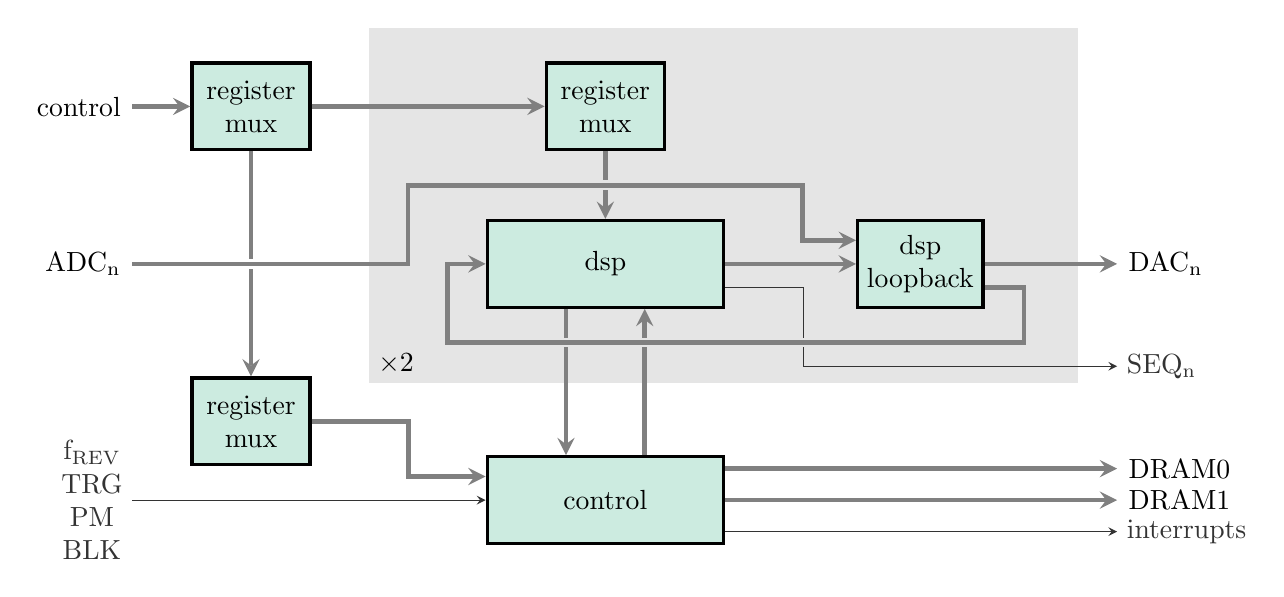
\begin{tikzpicture}

    \path
        node [background fill,
            minimum width=9cm, minimum height=4.5cm] (gen dsp) {};
    \node [above right] at (gen dsp.south west) {$\times2$};

    \path (gen dsp.north)
        ++(-1.5,-1) node [box] (dsp registers) {register\\mux}
        +(-4.5,0) node [box] (top registers) {register\\mux}
        ++(0,-2) node [box, minimum width=3cm] (dsp) {dsp}
        +(4,0) node [box] (loopback) {dsp\\loopback}
        +(0,-3) node [box, minimum width=3cm] (control) {control};
    \path (top registers)
        ++(0,-4) node [box] (control registers) {register\\mux};
    \path (dsp-|gen dsp.west) coordinate (adc in);

    % Register wiring
    \draw [bus] (top registers) -- (dsp registers);
    \draw [bus] (dsp registers) -- (dsp);
    \draw [bus] (top registers) -- (control registers);
    \draw [bus] (control registers)
        -- ++(2,0) |- ($(control.west)+(0,0.3)$);

    % Main DSP wiring
    \draw [bus] (dsp) -- (loopback);
    \draw [bus] (loopback) -- ++(2.5,0)
        coordinate (dac out)
        node [anchor=west] {DAC\textsubscript{n}};
    \draw [bus] ([xshift=-5mm]dsp.south) -- (\lastcoord|-control.north);
    \draw [bus] ([xshift=5mm]control.north) -- (\lastcoord|-dsp.south);
    \draw [trigger line, ->]
        ($(dsp.east)+(0,-0.3)$) -- ++(1,0) -- ++(0,-1)
        -- (\lastcoord-|dac out)
        node [anchor=west] {SEQ\textsubscript{n}};

    % ADC loopback wiring
    \multipath [bus, multipath background=background colour]
        {\draw (adc in)
            -- ++(0.5,0) -- ++(0,1) -- ($(loopback)+(-1.5,1)$)
            |- ($(loopback.west)+(0,0.3)$);}
    \multipath [bus, multipath background=background colour]
        {\draw ($(loopback.east)+(0,-0.3)$)
            -- ++(0.5,0) -- ++(0,-0.7)
            -| ($(adc in)+(1,0)$) -- (dsp);}
    \multipath [bus, -] {\draw (adc in) -- +(-3,0)
        node [anchor=east] {ADC\textsubscript{n}};}

    % Move (adc in)
    \path (adc in) -- +(-3,0) coordinate (adc in);

    % Control I/O
    \draw [bus] ($(control.east)+(0,0.4)$) -- (\lastcoord-|dac out)
        node [anchor=west] {DRAM0};
    \draw [bus] (control.east) -- (\lastcoord-|dac out)
        node [anchor=west] {DRAM1};
    \draw [trigger line, ->]
        ($(control.east)+(0,-0.4)$) -- (\lastcoord-|dac out)
        node [anchor=west] {interrupts};
    \draw [trigger line, <-]
        (control) -- (control-|adc in)
        node [anchor=east] {f\textsubscript{REV}\\TRG\\PM\\BLK};
    \draw [bus] (adc in|-top registers)
        node [anchor=east] {control}
        -- (top registers);

\end{tikzpicture}

% vim: filetype=tex:

\end{centering}
\end{figure}

\begin{figure}[ht]
\begin{centering}
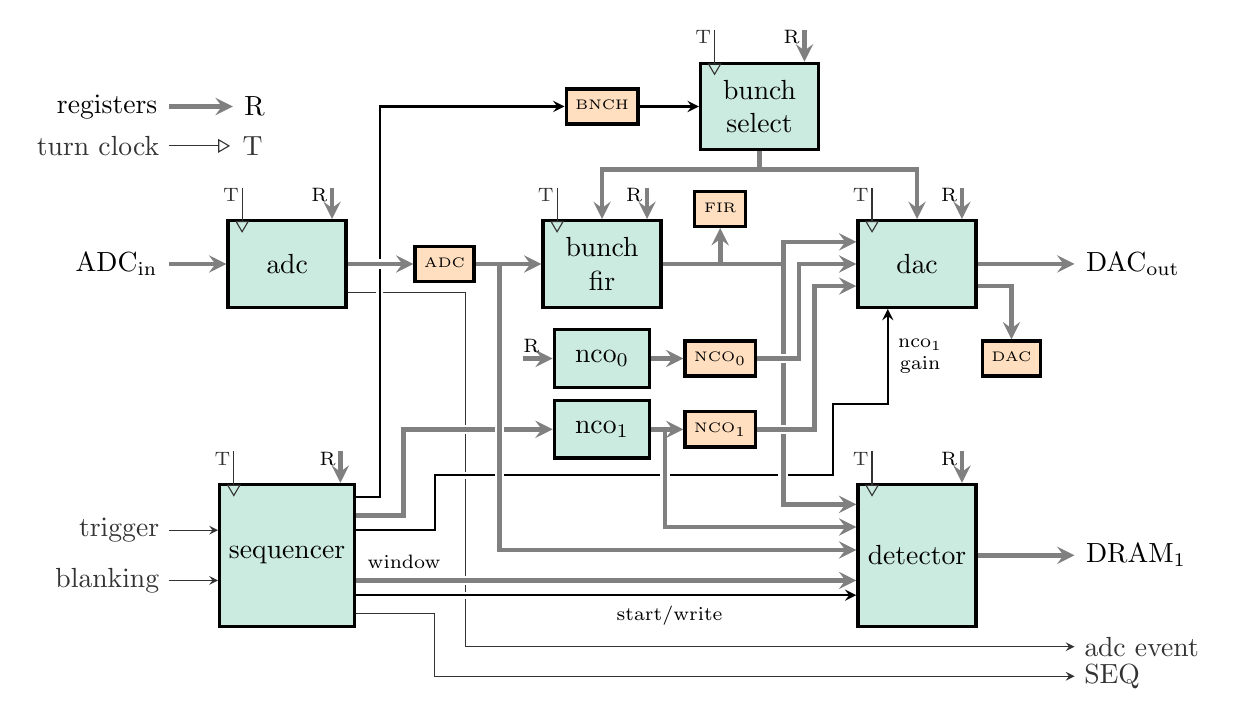
\begin{tikzpicture}[
    control/.style={
        draw, rectangle, very thick, accent fill,
        font=\tiny\strut,},
    nco box/.style={
        draw, rectangle, very thick, highlight fill,
        inner sep=0.75em},
    ]

    % Basic skeleton
    \path
        (0,0) node [box] (adc) {adc}
        +(0,-37mm) node [box, minimum height=18mm] (sequencer) {sequencer}
        +(2cm,0)  node [control] (adc mux) {ADC}
        ++(4cm,0) node [box] (fir) {bunch\\fir}
        +(15mm,7mm) node [control] (fir out) {FIR}
        +(2cm,2cm) node [box] (bunch) {bunch\\select}
        +(0,2cm) node [control] (bunch mux) {BNCH}
        ++(0,-12mm) node [nco box] (nco0) {nco\textsubscript{0}}
        +(15mm,0) node [control] (nco0 mux) {NCO\textsubscript{0}}
        ++(0,-9mm) node [nco box] (nco1) {nco\textsubscript{1}}
        +(15mm,0) node [control] (nco1 mux) {NCO\textsubscript{1}}
        (fir)
        ++(4cm,0) node [box] (dac) {dac}
        +(12mm,-12mm) node [control] (dac out) {DAC}
        ++(0,-37mm) node [box, minimum height=18mm] (detector) {detector};

    \draw [bus, <-]
        (adc) -- +(-15mm,0) coordinate (inputs)
        node [anchor=east] {ADC\textsubscript{in}};
    \draw [bus]
        (dac) -- +(20mm,0) coordinate (outputs)
        node [anchor=west] {DAC\textsubscript{out}};
    \draw [bus] (dac.-20) -| (dac out);

    \draw [trigger line, ->]
        (adc.-25) -- ++(15mm,0) -- ++(0,-45mm) -- (\lastcoord-|outputs)
        node [anchor=west] {adc event};

    \multipath [thick, ->] {\draw
        (sequencer.20) -- ++(10mm,0) -- ++(0,7mm)
        -| ($(detector.north west)+(-3mm,10mm)$)
        -| ($(dac.south west)+(4mm,0)$)
        node [pos=0.75, anchor=west, font=\scriptsize]
            {nco\textsubscript{1}\\gain};}

    \draw [bus] (bunch) -- ++(0,-8mm) -| (fir);
    \draw [bus] (bunch) -- ++(0,-8mm) -| (dac);
    \draw [thick, ->] (bunch mux) -- (bunch);

    \multipath [bus] {
        \draw (fir) -| (fir out);
        \draw (fir) -- +(23mm,0) |- (dac.160);
        \draw (fir) -- +(23mm,0) |- (detector.140);}

    \draw [bus] (nco0) -- (nco0 mux);
    \multipath [bus] {\draw (nco0 mux) -- +(10mm,0) |- (dac);}
    \multipath [bus] {\draw (nco1 mux) -- +(12mm,0) |- (dac.-160);}
    \multipath [bus] {
        \draw (nco1) -- (nco1 mux);
        \draw (nco1) -- +(8mm,0) |- (detector.155);}

    \draw [trigger line, <-] (sequencer.160) -- (inputs|-sequencer.160)
        node [anchor=east] {trigger};
    \draw [trigger line, <-] (sequencer.-160) -- (inputs|-sequencer.-160)
        node [anchor=east] {blanking};
    \multipath [thick, ->] {\draw (sequencer.40) -- +(3mm,0) |- (bunch mux);}
    \multipath [bus] {\draw (sequencer.30) -- +(6mm,0) |- (nco1);}
    \multipath [bus] {\draw
        (sequencer.-20) -- (\lastcoord-|detector.west)
        node [pos=0, anchor=south west, font=\scriptsize] {window};}
    \multipath [thick, ->] {\draw
        (sequencer.-30) -- (\lastcoord-|detector.west)
        node [pos=0.5, anchor=north west, font=\scriptsize] {start/write};}
    \draw [trigger line, ->] (sequencer.-40)
        -- ++(10mm,0) -- ++(0,-8mm) -- (\lastcoord-|outputs)
        node [anchor=west] {SEQ};

    \draw [bus] (detector) -- (detector-|outputs)
        node [anchor=west] {DRAM\textsubscript{1}};

    \multipath [bus] {
        \draw (adc) -- (adc mux);
        \draw (adc mux) -- (fir);
        \draw (adc mux) -- +(7mm,0) |- (detector.175);}

    \draw [trigger]
        (inputs) ++(0,15mm)
        node [anchor=east] {turn clock}
        -- ++(6mm,0) node [anchor=west] at +(6pt,0) {T};
    \draw [bus]
        (inputs) ++(0,20mm)
        node [anchor=east] {registers}
        -- ++(6mm+6pt,0) node [anchor=west] {R};
    \draw [bus, <-] (nco0) -- +(-10mm,0)
        node [anchor=south west, font=\scriptsize,
            inner xsep=0, inner ysep=2pt, line width=0pt] {R};
    \foreach \x in {adc, fir, dac, bunch, sequencer, detector} {
        \draw [trigger] (\x.north west)
            ++(2mm,4mm)
            node [anchor=north east, font=\scriptsize,
                inner xsep=1pt, inner ysep=0pt] {T}
            -- +(0,-4mm);
        \draw [bus, <-] (\x.north east)
            ++(-2mm,0) -- +(0,4mm)
            node [thin, anchor=north east, font=\scriptsize,
                inner xsep=1.5pt, inner ysep=0pt] {R};
    };

\end{tikzpicture}

% vim: filetype=tex:

\end{centering}
\end{figure}

\begin{figure}[ht]
\begin{centering}
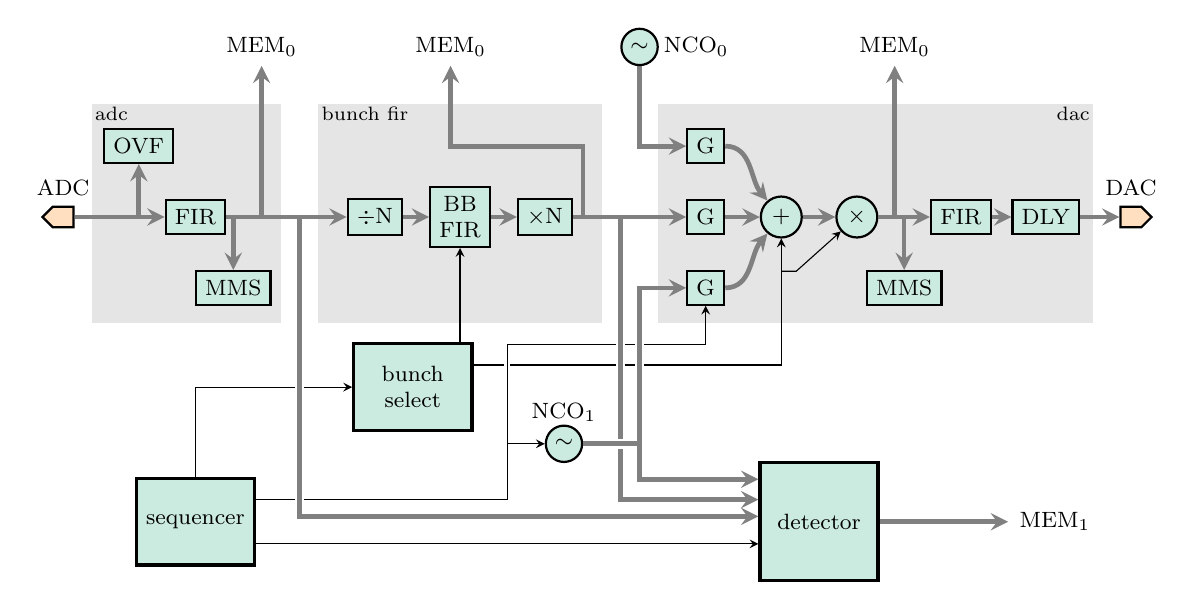
\begin{tikzpicture}[
    adc-dac/.style={
        draw, single arrow, thick, accent fill,
        single arrow head extend=0pt, shape border rotate=#1},
    area label/.style={anchor=north west, font=\scriptsize, inner sep=1pt},
    mul/.style={
        draw=black, circle, thick, highlight fill, inner sep=0.5ex},
    every node/.append style={font=\footnotesize},
    control mux/.style={
        small box, accent fill, label={[font=\tiny]above:MUX}, font=\tiny},
    x=12mm, y=9mm
    ]

    \path [background fill] (0.3,1.6)
        node [area label] {adc} rectangle ++(2,-3.1);
    \path [background fill] (2.7,1.6)
        node [area label] {bunch fir} rectangle ++(3.0,-3.1);
    \path [background fill] (6.3,1.6) rectangle ++(4.6,-3.1)
        ++(0,3.1) node [area label, anchor=north east] {dac};

    \path
        (0,0) node [adc-dac=180, label={ADC}] (adc in) {}
        +(0.8,1) node [small box] (adc ovf) {OVF}
        ++(1.4,0) node [small box] (adc fir) {FIR}
        +(0.4,-1) node [small box] (adc mms) {MMS}
        +(0.7,2.4) node (adc mem) {MEM\textsubscript{0}}
        ++(1.9,0) node [small box] (decimate) {$\div$N}
        ++(0.9,0) node [small box] (bb fir) {BB\\FIR}
        ++(0.9,0) node [small box] (interpolate) {$\times$N}
        +(-1,2.4) node (fir mem) {MEM\textsubscript{0}}
        ++(1.7,0) node [small box] (fir gain) {G}
        +(0,1) node [small box] (nco0 gain) {G}
        +(0,-1) node [small box] (nco1 gain) {G}
        ++(0.8,0) node [mul] (sum) {$+$}
        ++(0.8,0) node [mul] (product) {$\times$}
        +(0.5,-1) node [small box] (dac mms) {MMS}
        +(0.4,2.4) node (dac mem) {MEM\textsubscript{0}}
        ++(1.1,0) node [small box] (dac fir) {FIR}
        ++(0.9,0) node [small box] (delay) {DLY}
        ++(0.9,0) node [adc-dac, label={DAC}] (dac out) {};

    \node [box] at (1.4,-4.3) (sequencer) {sequencer};
    \path (bb fir) ++(-0.5,-2.4) node [box] (bunch) {bunch\\select};
    \node [box, minimum height=15mm] at (8,-4.3) (detector) {detector};
    \path (nco1 gain) ++(-1.5,-2.2)
        node [mul,
            label={[inner sep=1pt]above:NCO\textsubscript{1}}] (nco1) {$\sim$};

    \draw [bus] (adc in) -- (adc fir);
    \draw [bus] (adc in) -| (adc ovf);
    \draw [bus] (adc fir) -| (adc mms);
    \draw [bus] (adc fir) -| (adc mem);
    \draw [bus] (adc fir) -- (decimate);

    \draw [bus] (decimate) -- (bb fir);
    \draw [bus] (bb fir) -- (interpolate);
    \draw [bus] (interpolate) -- (fir gain);
    \draw [bus] (interpolate) ++(0.4,0) -- ++(0,1) -| (fir mem);
    \draw [bus] (fir gain) -- (sum);
    \draw [bus] (nco0 gain) to [out=0, in=130] (sum);
    \draw [bus] (nco1 gain) to [out=0, in=-130] (sum);
    \draw [bus] (sum) -- (product);
    \draw [bus] (product) -- (dac fir);
    \draw [bus] (product) -| (dac mms);
    \draw [bus] (product) -| (dac mem);
    \draw [bus] (dac fir) -- (delay);
    \draw [bus] (delay) -- (dac out);

    \draw [bus, <-] (nco0 gain) -- ++(-0.7,0) -- ++(0,1.4)
        node [mul, label={[inner sep=1pt]right:NCO\textsubscript{0}}] {$\sim$};

    \draw [thin, ->] (sequencer) |- (bunch);
    \draw [thin, ->] (bunch.north-|bb fir) -- (bb fir);
    \draw [thin, <-] (product) -- ++(-130:1) -- (\lastcoord-|sum);
    \draw [thin, ->] (bunch.20) -| (sum);
    \draw [thin, ->] (sequencer.-20) -- (\lastcoord-|detector.west);
    \draw [thin, ->] (sequencer.20) -| ($(nco1)+(-0.6,0)$)
        coordinate (nco1 control) -- (nco1);
    \multipath [thin] {\draw (nco1 control) -- ++(0,1.4);}
    \draw [thin, ->] (nco1 control) -- ++(0,1.4) -| (nco1 gain);

    \multipath [bus] {\draw (interpolate) ++(0.8,0) |- (detector.160);}
    \multipath [bus] {\draw (adc fir) ++(1.1,0) |- (detector.175);}
    \multipath [bus, -] {
        \draw (nco1) -- ++(0.8,0) -- (\lastcoord|-nco1 gain);
        \draw (nco1) -- ++(0.8,0) -- (\lastcoord|-detector.145);
    }
    \draw [bus] (nco1) ++(0.8,0) |- (nco1 gain);
    \draw [bus] (nco1) ++(0.8,0) |- (detector.145);

    \draw [bus] (detector) -- ++(2,0)
        node [anchor=west] {MEM\textsubscript{1}};

\end{tikzpicture}

% vim: filetype=tex:

\end{centering}

% \begin{tabularx}{\textwidth}{cXcX}
%     \tikz [inline text] \node [small box] {OVF}; &
%     Overflow detection.
% \\
%     \tikz [inline text] \node [small box] {MMS}; &
%     Min/Max/Sum: computes mean bunch positions, peak to peak bunch motion, and
%     standard deviation of bunch motion.
% \\
% \end{tabularx}

% This figure shows the overall data processing path for a single channel.  Data
% from the ADC is first checked for overflow and is passed through a short
% compensation filter (first FIR).  The resulting ADC input stream is available
% for capture to memory (MEM\textsubscript{0}), and can be used for tune
% measurement in the detector.  The MMS (Min/Max/Sum) block measures the average
% bunch position, and both the peak-to-peak and standard deviation of bunch
% motion.
\end{figure}


\end{document}
